\begin{block}{QSVM Results}
    Legend of labels: \textbf{D-Wave} represents the quantum solution, \textbf{CPLEX} represents the classical implementation of SVM, \textbf{RoBERTa} represents the Transformer architecture.

    \begin{figure}[h!]
        \centering
        \begin{minipage}{0.3\textwidth}
            \centering
            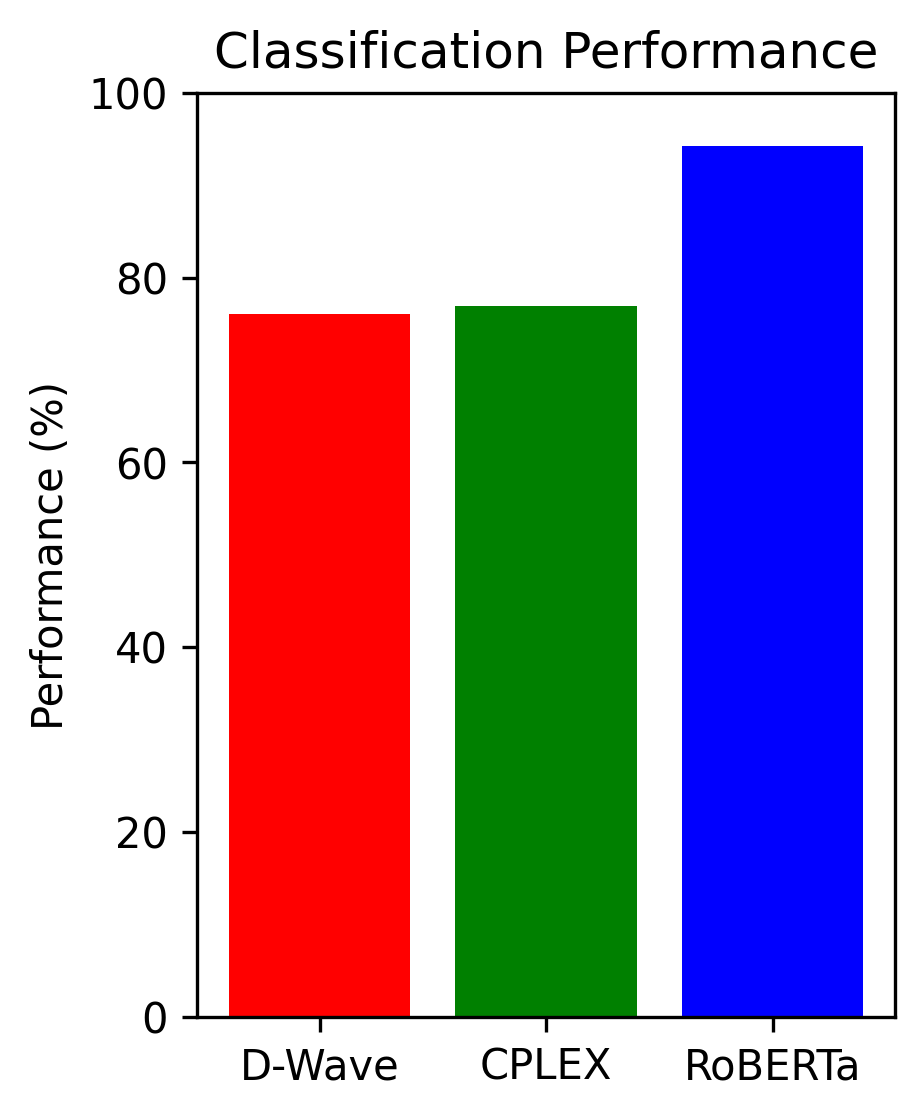
\includegraphics[height=0.14\textheight]{logos/performance.png}
        \end{minipage}%
        \hfill
        \begin{minipage}{0.65\textwidth}
            \begin{alertblock}{Classification Performance}
                RoBERTa is almost 20\% better than D-Wave and CPLEX, which classify 75\% of cases correctly.
            
                CPLEX is slightly better than D-Wave due to some limitations of the current hybrid solvers, which restrict the domain of the optimisation variables from real numbers to integers.
            \end{alertblock}
        \end{minipage}
    \end{figure}

    \begin{figure}[h!]
        \centering
        \begin{minipage}{0.65\textwidth}
            \begin{alertblock}{Training Time}
                The time required by D-Wave to find an optimal assignment is 60\% less than that of CPLEX. 

                Although not available, it is reasonable to expect an even better result if compared to the time required by RoBERTa, which we can fairly expect to amount to several hours of training on high-performance machines.
            \end{alertblock}
        \end{minipage}%
        \hfill
        \begin{minipage}{0.3\textwidth}
            \centering
            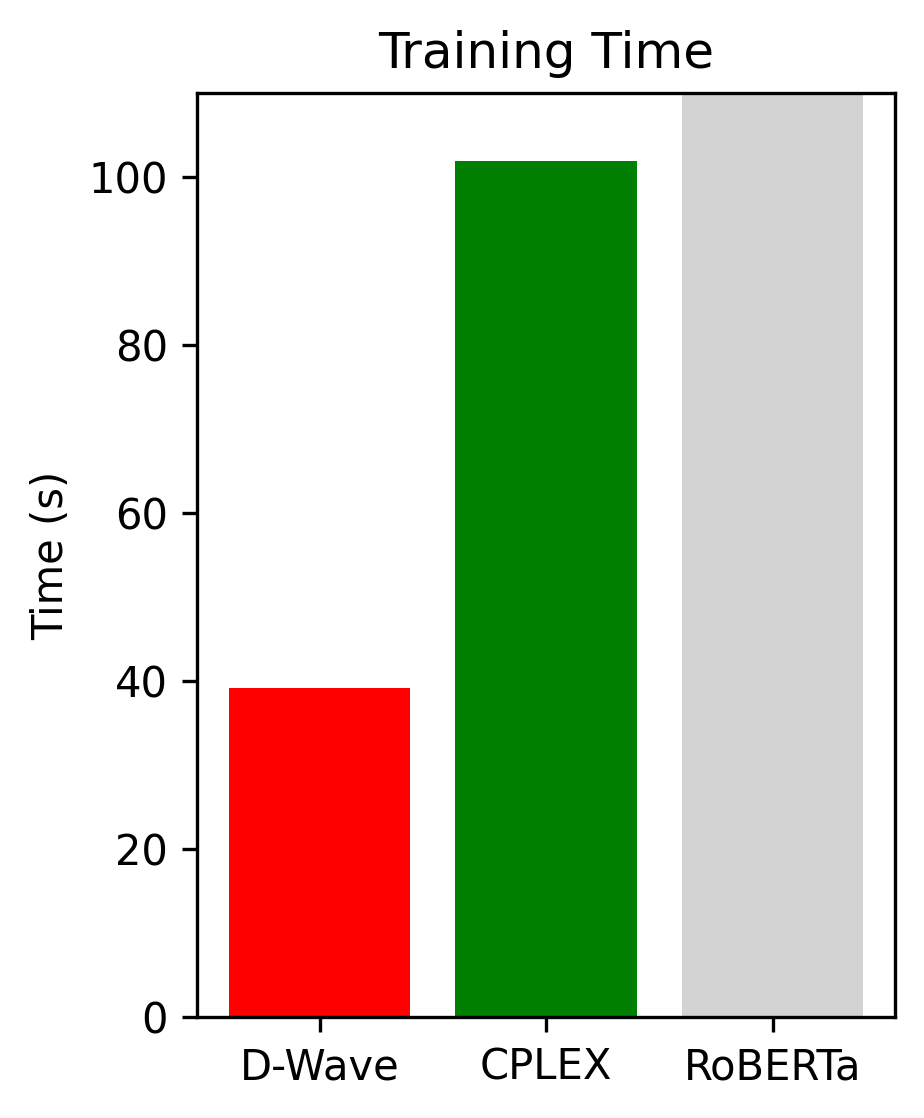
\includegraphics[height=0.14\textheight]{logos/training.png}
        \end{minipage}
    \end{figure}

    \begin{figure}[h!]
        \centering
        \begin{minipage}{0.3\textwidth}
            \centering
            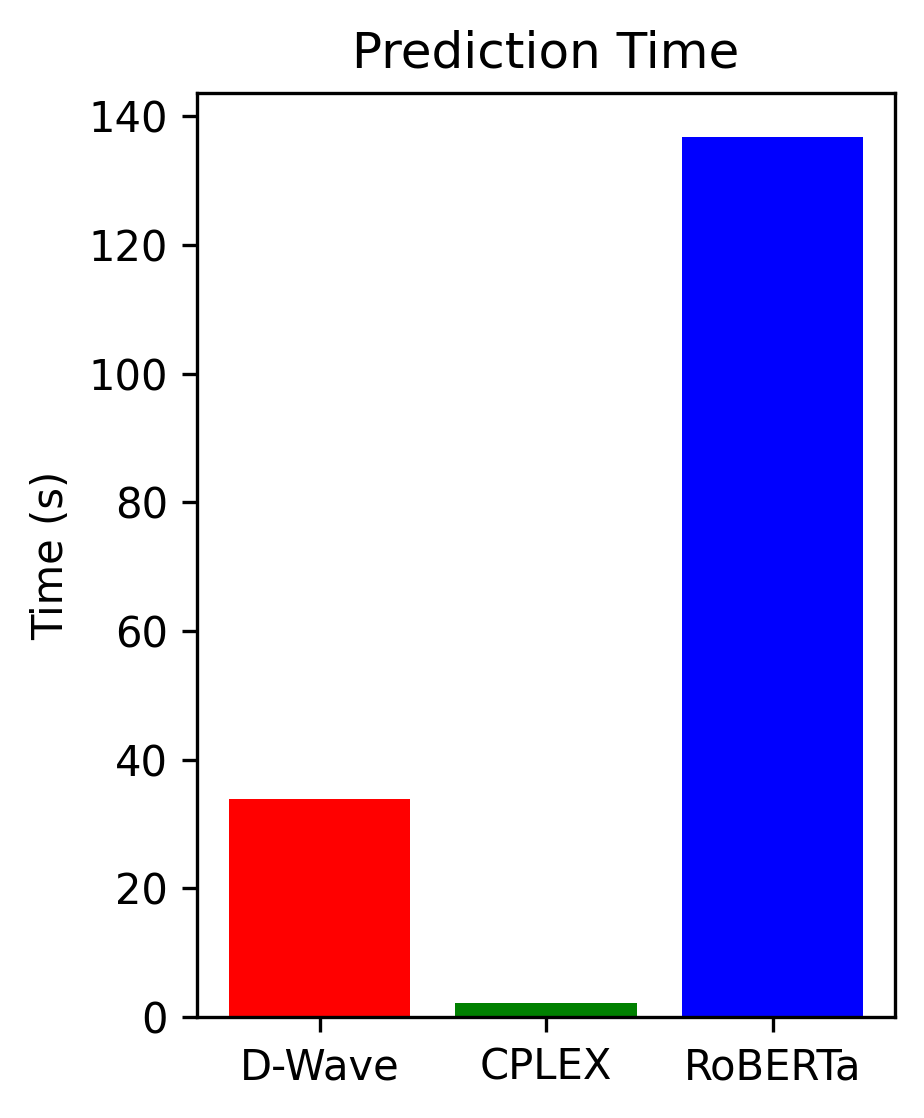
\includegraphics[height=0.14\textheight]{logos/prediction.png}
        \end{minipage}%
        \hfill
        \begin{minipage}{0.65\textwidth}
            \begin{alertblock}{Prediction Time}
                The complexity of the RoBERTa architecture also affects the time required for prediction.

                The longer time D-Wave requires is due to the resolution methodology, which returns a set of optimal solutions from which a majority vote is taken during inference.

                Experimentally, we find that it is possible to use only the first of the optimal assignments produced, reducing the time to values comparable to those of CPLEX.
            \end{alertblock}
        \end{minipage}
    \end{figure}
\end{block}